\documentclass[a4paper]{article}

\usepackage[table]{xcolor}%this has to be the first!!!!!!
\usepackage{fullpage} % Package to use full page
%\usepackage{parskip} % Package to tweak paragraph skipping
\usepackage{tikz} % Package for drawing
\usetikzlibrary{shapes,arrows,matrix,positioning}
\usepackage{amsmath}
\usepackage{indentfirst}
\usepackage{hyperref}
\usepackage{subcaption}
\usepackage{graphics}
\usepackage{graphicx}
\usepackage{minted}
\usepackage{multicol}
\usepackage{mathrsfs}
%color define
\definecolor{codebg}{RGB}{230,255,253}
\definecolor{function}{RGB}{210,0,26}
\definecolor{para}{RGB}{255,137,137}
\definecolor{output}{RGB}{238,224,201}
\setminted[cpp]{mathescape=true,breaklines,bgcolor=codebg,linenos}

\tikzset{
  block/.style = {rectangle, draw, fill=output, text width=6cm, text centered, rounded corners, minimum height=4em},
  line/.style = {draw, -latex'},
}


%function newcommand
\newcommand{\func}[1]{\textbf{\textcolor{function}{#1}}}
\newcommand{\para}[1]{\textbf{\emph{\textcolor{para}{#1}}}}
\newcommand{\target}{\tikz \fill[brown] (2pt,2pt) rectangle (8pt,8pt);}
\newcommand{\activetest}{\tikz \fill[black] (3pt,3pt) circle (3pt);}
\newcommand{\prolong}{\tikz \fill[blue] (3pt,3pt) circle (3pt);}
\newcommand{\rest}{\tikz \fill[red] (3pt,3pt) circle (3pt);}

\usepackage{biblatex}
\addbibresource{bibliography.bib}
\title{viscosity.h Documentation}
\author{Haochen(Langford) Huang}
\date{\today}

\makeatletter%title setting
\def\@maketitle{%
  \newpage
  \null
  \vskip 2em%
  \begin{center}%
  \let \footnote \thanks
    {\LARGE \@title \par}%
    \vskip 1.5em%
    {\Large
      \lineskip .5em%
      \begin{tabular}[t]{c}%
        \@author
      \end{tabular}\par}%
    \vskip 1em%
    {\large \@date\par}%
    \vskip 1em%
    {\large version:1.0}%
  \end{center}%
  \par
  \vskip 1.5em}
\makeatother

\begin{document}

\maketitle

\section{Introduction and Background}
\textbf{viscosity.h} is constructed exclusively for NS solver 'centered.h' (see corresponding doc for more information.), whose purpose is to solve viscos equation implicitly using poisson equation solver built in 'poisson.h'. The governing equation is 
\begin{equation}\label{equ:desired}
  \rho_{n+ \frac{1}{2}}[ \frac{ \mathbf{u}^*- \mathbf{u}'}{\Delta t}] = \nabla\cdot [2\mu_{n+ \frac{1}{2}} \mathbf{D}^*]
\end{equation}
where $ \mathbf{D}^* = [\nabla \mathbf{u}^*+ (\nabla \mathbf{u}^*)^T]/2$, $ \mathbf{u}'$ is known variable and $ \mathbf{u}^*$ is the desired output.\par
Consider intergral form of equation \ref{equ:desired}
\begin{equation}
  \int_{\Omega}\rho_{n+ \frac{1}{2}} [ \frac{ \mathbf{u}^*- \mathbf{u}'}{\Delta t}]dV = \int_{\Omega}\nabla\cdot[2\mu_{n+ \frac{1}{2}} \mathbf{D}^*] dV = \int_{\partial \Omega} [2\mu_{n+ \frac{1}{2}} \mathbf{D}^*]\cdot \mathbf{n}dS
\end{equation}
The discrete form of this equation reads (component form is presented instead of tensor for sake of convenience).
\begin{equation}\label{equ:discrete}
  \Delta \rho_{n+ \frac{1}{2}} [ \frac{u_i^*-u_i'}{\Delta t} ] = \sum_{f = 1}^6(n_f \mu_{n+ \frac{1}{2}}( \frac{\partial u_j^*}{\partial x_i}+ \frac{\partial u_i^*}{\partial x_j}))_f \quad i= x,y,z\quad j = normal(f)
\end{equation}
where $f$ in summation and subscript represents surfaces of single cell, $j$ represents coordinate component of face normal disregarding negative or positive direction, $n_f$ indicates whether the face normal is consistent with positive direction of coordinate, taking 2D cell as an example
\begin{figure}[H]
    \centering
    \begin{tikzpicture}[scale=0.8]
    \draw (-2.0,0)--(2.0,0)--(2.0,4)--(-2.0,4)--(-2.0,0);
    \node[left=2pt](a) at (-2.0,2.0) {$1$};
    \node[below=1pt](b) at (0,0) {$2$};
    \node[right=1pt](c) at (2.0,2.0) {$3$};
    \node[above=1pt](d) at (0,4.0) {$4$};
    \draw[->] (-2.5,0)--(2.5,0) node[anchor=west]{$x$};
    \draw[->] (-2.0,-0.5)--(-2.0,4.5) node[anchor=west]{$y$};
    \end{tikzpicture}
    \caption{2D cell example.}
    \label{fig:2Dexample}
\end{figure}
Unfold \emph{R.H.S.} of equation \ref{equ:discrete} based on 2D cell depicted by Fig.\ref{fig:2Dexample} yields
\begin{equation}\label{equ:2dunfold}
    \emph{R.H.S} = [\mu_3(\frac{\partial u^*_x}{\partial x_i}+\frac{\partial u^*_i}{\partial x})_3 - \mu_1(\frac{\partial u^*_x}{\partial x_i}+\frac{\partial u^*_i}{\partial x})_1+\mu_4(\frac{\partial u^*_y}{\partial x_i}+\frac{\partial u^*_i}{\partial y})_4-\mu_2(\frac{\partial u^*_y}{\partial x_i}+\frac{\partial u^*_i}{\partial y})_2]\quad i = x,y
\end{equation}
 Constructing derivative is simple for aligned direction but cumbersome for spliting direction.
\begin{figure}[H]
    \centering
    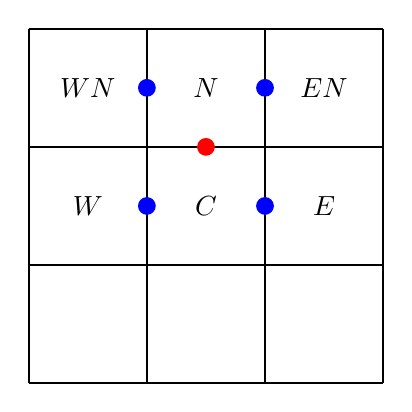
\begin{tikzpicture}[scale=1.5]
      \draw[step=1cm,thick] (0,0) grid (3.0,3.0);
      \node at (1.5,1.5) {$C$};
      \node at (2.5,1.5) {$E$};
      \node at (0.5,1.5) {$W$};
      \node at (1.5,2.5) {$N$};
      \node at (0.5,2.5) {$WN$};
      \node at (2.5,2.5) {$EN$};
      \filldraw[blue] (1.0,1.5) circle (2pt);
      \filldraw[blue] (2.0,1.5) circle (2pt);
      \filldraw[blue] (1.0,2.5) circle (2pt);
      \filldraw[blue] (2.0,2.5) circle (2pt);
      \filldraw[red] (1.5,2.0) circle (2pt);
    \end{tikzpicture}
    \caption{Sketch for derivative calculating.}
    \label{fig:2Dcelld}
\end{figure}
Still take $2D$ cell as an example, as shown in Fig.\ref{fig:2Dcelld}, aligned direction derivative \emph{e.g.}$(\frac{\partial u^*_y}{\partial y})_n$ (lower case indicates corresponding cell face) can be obtained by simply cnetral difference scheme
\begin{equation}
  (\frac{\partial u^*_y}{\partial x_y})_n = \frac{u^*_N-u^*_C}{\Delta}
\end{equation}
However, for splitting direction derivative \emph{e.g.}$(\frac{\partial u^*_y}{\partial x})_n$ highlighted by red point above, there is no direct method to calculate the desired but average the ambient derivatives (highlighted by blue point), which are obtained following the direct method.
\begin{equation}
  (\frac{\partial u^*_y}{\partial x})_n = \frac{ ( \frac{\partial u^*_y}{\partial x})_{wn}+( \frac{\partial u^*_y}{\partial x})_{en}+( \frac{\partial u^*_y}{\partial x})_{w}+( \frac{\partial u^*_y}{\partial x})_{e}}{4}
\end{equation}
Now consider constructing $x$ component of equation \ref{equ:discrete} for cell locates $(0,0)$. We herein denote $x,y$ components of $ \mathbf{u}$ as $u,v$ but not $u_x,u_y$ for sake of clarity. The \emph{L.H.S} can be directly expressed as 
\begin{equation}
  \emph{L.H.S}=\Delta\rho_{n+ \frac{1}{2}}[ \frac{u^*_{0,0}-u'_{0,0}}{\Delta t}]
\end{equation}
Then the first two terms of equation \ref{equ:2dunfold} which can be obtained directly are
\begin{equation}
  \emph{R.H.S}\,F2 =  2\mu_{(\frac{1}{2},0)}(\frac{u^*_{1,0}-u^*_{0,0}}{\Delta})-2\mu_{(-\frac{1}{2},0)}(\frac{u^*_{0,0}-u^*_{-1,0}}{\Delta})
\end{equation}
Finally the last two terms that is calculated by averaging yields
\begin{equation}
\begin{aligned}
  \emph{R.H.S}\,L2 = 
    \mu_{(0,\frac{1}{2})}[\frac{u^*_{(0,1)}-u^*_{(0,0)}}{\Delta}
    +\frac{v^*_{(1,1)}-v^*_{(-1,1)}+v^*_{(1,0)}-v^*_{(-1,0)}}{4\Delta}]\\-\mu_{(0,-\frac{1}{2})}[\frac{u^*_{(0,0)}-u^*_{(0,-1)}}{\Delta}+\frac{v^*_{(1,0)}-v^*_{(-1,0)}+v^*_{(1,-1)}-v^*_{(-1,-1)}}{4\Delta}]
\end{aligned}
\end{equation}
Rearrange the equations we have
\begin{equation}\label{equ:aim}
    u^*_{(0,0)} = \frac{\frac{\Delta t}{\rho}(2\mu_{(\frac{1}{2},0)}u^*_{(1,0)}+2\mu_{(-\frac{1}{2},0)}u^*_{(-1,0)}+\mathscr{A}-\mathscr{B})+\Delta^2 u'_{(0,0)}}{\Delta^2+\frac{\Delta t}{\rho}(2\mu_{(\frac{1}{2},0)}+2\mu_{(-\frac{1}{2},0)}+\mu_{(0,\frac{1}{2})}+\mu_{(0,-\frac{1}{2})})}
\end{equation}
where
\begin{gather}
    \mathscr{A} = \mu_{(0,\frac{1}{2})}(u^*_{(0,1)}+\frac{v^*_{(1,1)}+v^*_{(1,0)}-v^*_{(-1,1)}-v^*_{(-1,0)}}{4})\\
    \mathscr{B} = \mu_{(0,-\frac{1}{2})}(-u^*_{(0,-1)}+\frac{v^*_{(1,-1)}+v^*_{(1,0)}-v^*_{(-1,-1)}-v^*_{(1,0)}}{4})
\end{gather}
Now, we obtain the implicit discrete linear expressions for desired valuable $ \mathbf{u}^*$. Moreover, if we modify the governing equation into a more general form
\begin{equation}\label{equ:resi}
  \mathbf{u}' = \mathbf{u}^* - \frac{\Delta t\nabla\cdot[2 \mu_{n+ \frac{1}{2}} \mathbf{D}^*]}{\rho_{n + \frac{1}{2}}} = \mathscr{D}( \mathbf{u}^*)
\end{equation}
here $\mathscr{D}$ is a linear operator that satisfies
\begin{align}
  RES^k =& \mathbf{u}'- \mathscr{D}( \mathbf{u}^{*,k}) \\
  \mathscr{D}(\delta \mathbf{u}^{*,k}) =& RES^k \label{equ:delta}\\
  \mathbf{u}^{*,k+1} =& \mathbf{u}^{*,k}+ \delta\mathbf{u}^{*,k}
\end{align}
We denote by $k$ the $k$th iterate approximating result of corresponding value. Then the multicycle solver constructed in 'poisson.h' can be applied to solve viscosity equation with specific relaxation and residual functions, which are built in this headfile. 
\section{Functions}

\subsection{Define}

\subsubsection{Parameters}
\begin{center}
  \begin{tabular}{|c|c|c|c|c|}
    \hline
    Name & Data type & Status & Option & Representation (before/after)\\[0.5ex]
    \hline\hline
    \para{mu} & face vector & unchanged & compulsory & $\mu^{n+ \frac{1}{2}}$\\
    \hline
    \para{rho} & scalar & unchanged & compulsory & $ \rho^{n + \frac{1}{2}}$ \\
    \hline
    \para{dt} & double & unchanged & compulsory & $\Delta t$\\
    \hline
  \end{tabular}
\end{center}

\subsubsection{Program Workflow}
\begin{multicols}{2}
  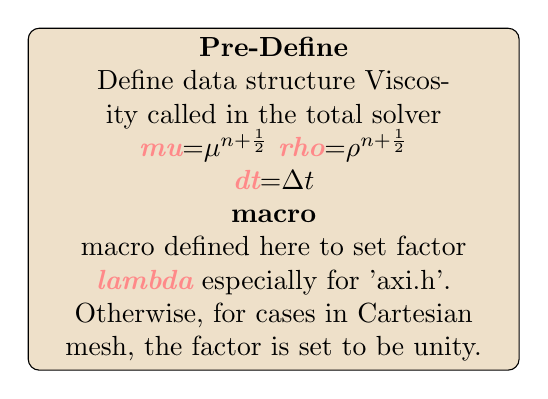
\begin{tikzpicture}
    \node [block](init){
        \textbf{Pre-Define}\\
        Define data structure Viscosity called in the total solver\\
        \para{mu}=$\mu^{n+ \frac{1}{2}}$ \para{rho}=$\rho^{n + \frac{1}{2}}$\\
        \para{dt}=$\Delta t$\\
        \textbf{macro}\\
        macro defined here to set factor \para{lambda} especially for 'axi.h'. Otherwise, for cases in Cartesian mesh, the factor is set to be unity. 
      };
  \end{tikzpicture}
  \columnbreak
  \begin{minted}[obeytabs=false,mathescape=true,breaklines]{cpp}
    #include "poisson.h"

    struct Viscosity {
      face vector mu;
      scalar rho;
      double dt;
    };

    #if AXI
    # define lambda ((coord){1., 1. + dt/rho[]*(mu.x[] + mu.x[1] + \
                  mu.y[] + mu.y[0,1])/2./sq(y)})
    #else // not AXI
    # if dimension == 1
    #   define lambda ((coord){1.})
    # elif dimension == 2
    #   define lambda ((coord){1.,1.})
    # elif dimension == 3
    #   define lambda ((coord){1.,1.,1.})
    #endif
    #endif
  \end{minted}
\end{multicols}

\subsection{\func{relax\_viscosity}}

\subsubsection{Parameters}
\begin{center}
  \begin{tabular}{|c|c|c|c|c|}
    \hline
    Name & Data type & Status & Option & Representation (before/after)\\[0.5ex]
    \hline\hline
    \rowcolor{output} \para{a} & scalar* & update & compulsory & $\delta \mathbf{u}^{*,k}/\delta \mathbf{u}^{*,k+1}$\\
    \hline
    \para{b} & scalar* & unchanged & compulsory & $RES$\\
    \hline
    \para{dt} & double & unchanged & compulsory & $\Delta t$\\
    \hline
    \para{l} & int & unchanged & compulsory &  mesh level \\
    \hline
    \para{data} & struct Vsicosity & unchanged & compulsory & $\mu^ {n+\frac{1}{2}}, \rho^{n+\frac{1}{2}}, \Delta t$ \\
    \hline
  \end{tabular}
\end{center}

\subsubsection{Worth Mentioning Details}
The purpose of this function is to implement equation \ref{equ:aim} and push forward iteration of G-S (or Jacobi) method for a single round on level $l$ mesh. Note the object processed is $\delta \mathbf{u}^{*}$ defined previously instead of $ \mathbf{u}^{*}$. Therefore, the equation it solves is equation \ref{equ:delta} with given residual $RES$ computed in another function.\par 
The Basilisk self-defined macro \mintinline{cpp}{foreach_level_or_leaf(l)} takes $l$ as its parameter and traverses each cell on level $l$ or leaf cell (the cell that cannot be divided) whose level is less than $l$. Interested readers are referred to 'poisson.h Documentation' or Van Hooft \emph{et.al.}\cite{van2018towards} for more information about mesh heiarchy in Basilisk. 

\subsubsection{Program Workflow}
\begin{multicols}{2}
  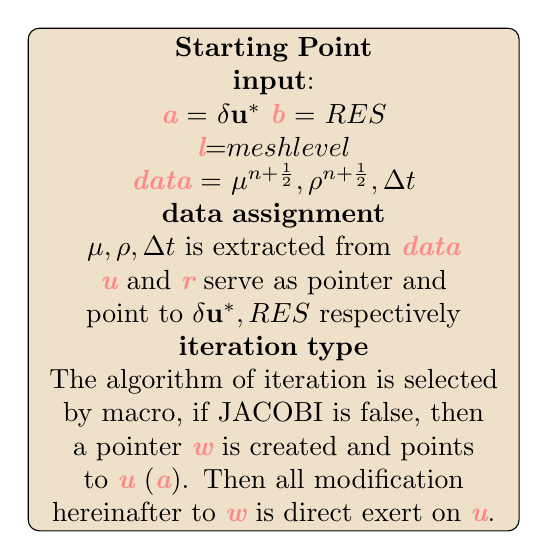
\begin{tikzpicture}
    \node [block](init){
        \textbf{Starting Point}\\
        \textbf{input}: \\
        \para{a} = $\delta \mathbf{u}^{*}$ \para{b} = $RES$\\ \para{l}=$mesh level$\\ \para{data} = $\mu^ {n+\frac{1}{2}}, \rho^{n+\frac{1}{2}}, \Delta t$\\
        \textbf{data assignment}\\
        $\mu,\rho,\Delta t$ is extracted from \para{data}\\
        \para{u} and \para{r} serve as pointer and point to $ \delta \mathbf{u}^{*}, RES$ respectively\\
        \textbf{iteration type}\\
        The algorithm of iteration is selected by macro, if JACOBI is false, then a pointer \para{w} is created and points to \para{u} (\para{a}). Then all modification hereinafter to \para{w} is direct exert on \para{u}.
      };
  \end{tikzpicture}
  \columnbreak
  \begin{minted}[obeytabs=false,mathescape=true,breaklines]{cpp}
    static void relax_viscosity (scalar * a, scalar * b, int l, void * data)
    {
      struct Viscosity * p = (struct Viscosity *) data;
      (const) face vector mu = p->mu;
      (const) scalar rho = p->rho;
      double dt = p->dt;
      vector u = vector(a[0]), r = vector(b[0]);

    #if JACOBI
      vector w[];
    #else
      vector w = u;
    #endif
  \end{minted}
\end{multicols}

\begin{center}
  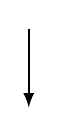
\begin{tikzpicture}
    \draw[-latex,thick](0,0) -- (0,-1); 
  \end{tikzpicture}
\end{center}
\newpage
\begin{multicols}{2}
  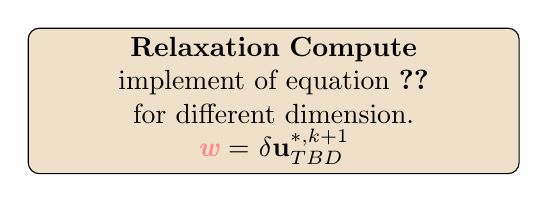
\begin{tikzpicture}
    \node [block](init){
        \textbf{Relaxation Compute}\\
        implement of equation \ref{equ:aim} for different dimension.\\
        \para{w} = $ \delta\mathbf{u}^{*,k+1}_{TBD}$\\
      };
  \end{tikzpicture}
  \columnbreak
  \begin{minted}[obeytabs=false,mathescape=true,breaklines]{cpp}
  foreach_level_or_leaf (l) {
    foreach_dimension()
     w.x[] = (dt/rho[]*(2.*mu.x[1]*u.x[1] + 2.*mu.x[]*u.x[-1]
#if dimension > 1
     + mu.y[0,1]*(u.x[0,1] +
      (u.y[1,0] + u.y[1,1])/4. -
      (u.y[-1,0] + u.y[-1,1])/4.)
     - mu.y[]*(- u.x[0,-1] +
         (u.y[1,-1] + u.y[1,0])/4. -
         (u.y[-1,-1] + u.y[-1,0])/4.)
#endif
#if dimension > 2
     + mu.z[0,0,1]*(u.x[0,0,1] +
        (u.z[1,0,0] + u.z[1,0,1])/4. -
        (u.z[-1,0,0] + u.z[-1,0,1])/4.)
     - mu.z[]*(- u.x[0,0,-1] +
         (u.z[1,0,-1] + u.z[1,0,0])/4. -
         (u.z[-1,0,-1] + u.z[-1,0,0])/4.)
#endif
     ) + r.x[]*sq(Delta))/
(sq(Delta)*lambda.x + dt/rho[]*(2.*mu.x[1] + 2.*mu.x[]
#if dimension > 1
     + mu.y[0,1] + mu.y[]
#endif
#if dimension > 2
     + mu.z[0,0,1] + mu.z[]
#endif
			     ));
  }
  \end{minted}
\end{multicols}

\begin{center}
  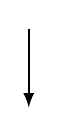
\begin{tikzpicture}
    \draw[-latex,thick](0,0) -- (0,-1); 
  \end{tikzpicture}
\end{center}

\begin{multicols}{2}
  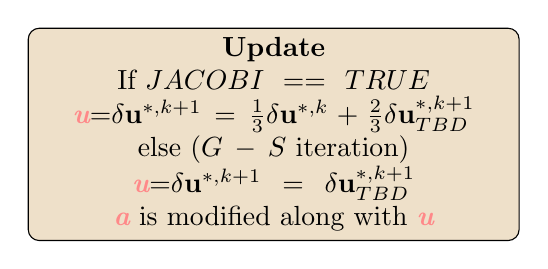
\begin{tikzpicture}
    \node [block](init){
        \textbf{Update}\\
        If $JACOBI==TRUE$\\
        \para{u}=$\delta \mathbf{u}^{*,k+1} = \frac{1}{3}\delta \mathbf{u}^{*,k}+ \frac{2}{3}\delta \mathbf{u}^{*,k+1}_{TBD}$\\
        else ($G-S$ iteration)\\
        \para{u}=$\delta \mathbf{u}^{*,k+1} = \delta \mathbf{u}^{*,k+1}_{TBD}$\\
        \para{a} is modified along with \para{u}\\
      };
  \end{tikzpicture}
  \columnbreak
  \begin{minted}[obeytabs=false,mathescape=true,breaklines]{cpp}
  #if JACOBI
    foreach_level_or_leaf (l)
      foreach_dimension()
        u.x[] = (u.x[] + 2.*w.x[])/3.;
  #endif
  
  #if TRASH
    vector u1[];
    foreach_level_or_leaf (l)
      foreach_dimension()
        u1.x[] = u.x[];
    trash ({u});
    foreach_level_or_leaf (l)
      foreach_dimension()
        u.x[] = u1.x[];
  #endif
  }
  \end{minted}
\end{multicols}

\subsection{\func{residual\_viscosity}}\label{sec:resi}
\subsubsection{Parameters}
\begin{center}
  \begin{tabular}{|c|c|c|c|c|}
    \hline
    Name & Data type & Status & Option & Representation (before/after)\\[0.5ex]
    \hline\hline
    \para{a} & scalar* & unchanged & compulsory & $ \mathbf{u}^{*,k}$\\
    \hline
    \para{b} & scalar* & unchanged & compulsory & $ \mathbf{u}'$\\
    \hline
    \rowcolor{output}\para{resl} & scalar* & \textbf{output} & compulsory & $RES^k = \mathbf{u}'- \mathscr{D}( \mathbf{u}^{*,k})$\\
    \hline
    \para{data} & struct Vsicosity & unchanged & compulsory & $\mu^ {n+\frac{1}{2}}, \rho^{n+\frac{1}{2}}, \Delta t$ \\
    \hline
  \end{tabular}
\end{center}
\subsubsection{Worth Mentioning Details}
This function updates residual by solving equation \ref{equ:resi} and returns the maximum component. Two computational methods are provided for tree and non-tree grid. The first method for tree grid costs more computational resource compared with the second one due to extra traversal or cell face but preserves 2nd order on tree grid. While the second method is of 2nd order with caresian but 1st with tree grid.\par
Consider quadtree for 2D cases shown in Fig.\ref{fig:cellandface} where coarser grid is of level $l$ and finer grid is of level $l+1$. $\target$ represents example targert cell whose residual will be compute to display the difference between two methods. $\activetest$ represents active point located at cell center where stores value for each cell. $\rest$ and $\prolong$ are ghost cells which do not exist initially. $\prolong$ is caculated by bilinear interpolation and is called as adjacent cell for finer cell while $\rest$ is obtained by averaging and is called from coarser cell. Moreover, cell faces highlighted by letters is another issue that woth mentioning. As can be seen from figure, target cell has five marked faces instead of four that face $A$ is divided into subfaces $A_1$ and $A_2$ due to tree grid. However when called face value from centered cell perspective \emph{i.e.} invoke value on face $A$ from target cell, the value returned is the average of $A_1$ and $A_2$. 

\begin{figure}[H]
    \centering
    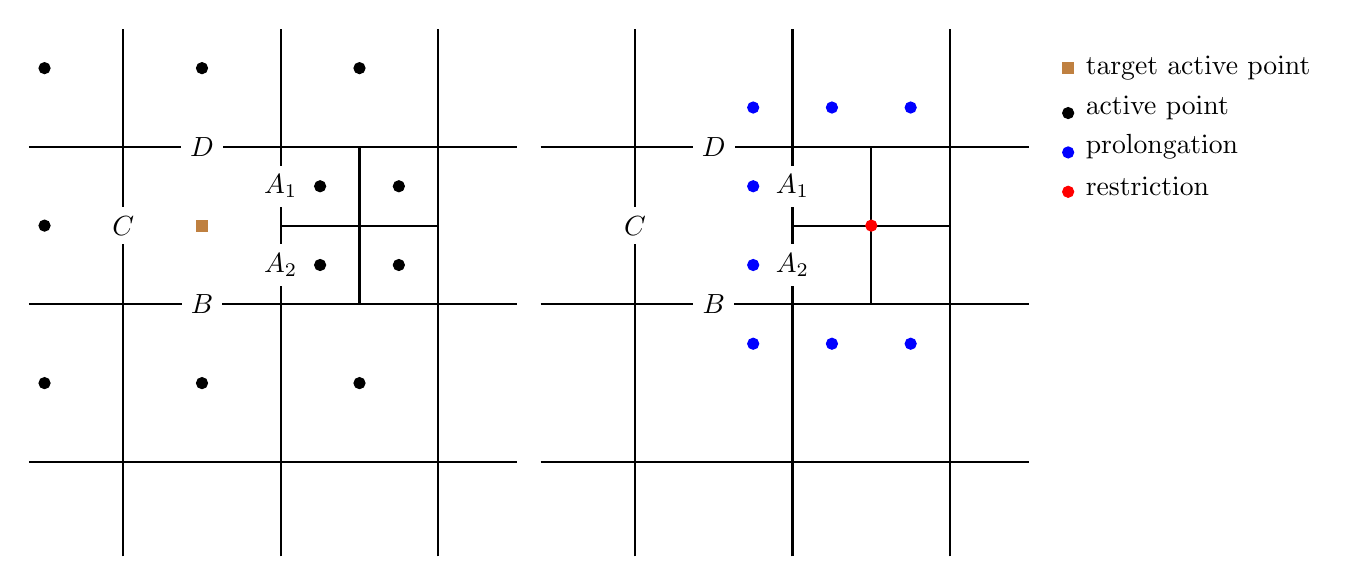
\begin{tikzpicture}
      \draw[thick,step=2cm] (-1.2,-1.2) grid (5.0,5.5); 
      \draw[thick,step=1cm] (2.0,2.0) grid (4.0,4.0); 
      \node[fill=white] at (2.0,3.5){$A_1$} ;
      \node[fill=white] at (2.0,2.5){$A_2$} ;
      \node[fill=white] at (1.0,2.0){$B$} ;
      \node[fill=white] at (0.0,3.0){$C$} ;
      \node[fill=white] at (1.0,4.0){$D$} ;
      \filldraw[brown] (1.0cm-2pt,3.0cm-2pt) rectangle (1.0cm+2pt,3.0cm+2pt);
      \filldraw[black] (1.0,1.0) circle (2pt);
      \filldraw[black] (3.0,1.0) circle (2pt);
      \filldraw[black] (-1.0,1.0) circle (2pt);
      \filldraw[black] (-1.0,3.0) circle (2pt);
      \filldraw[black] (-1.0,5.0) circle (2pt);
      \filldraw[black] (1.0,5.0) circle (2pt);
      \filldraw[black] (3.0,5.0) circle (2pt);
      \foreach \x in {2.5cm,3.5cm}
        \foreach \y in {2.5cm,3.5cm}
          \filldraw[black] (\x,\y) circle (2pt);

      \begin{scope}[xshift=6.5cm]
        \draw[thick,step=2cm] (-1.2,-1.2) grid (5.0,5.5); 
        \draw[thick,step=1cm] (2.0,2.0) grid (4.0,4.0); 
        \node[fill=white] at (2.0,3.5){$A_1$} ;
        \node[fill=white] at (2.0,2.5){$A_2$} ;
        \node[fill=white] at (1.0,2.0){$B$} ;
        \node[fill=white] at (0.0,3.0){$C$} ;
        \node[fill=white] at (1.0,4.0){$D$} ;
        %\filldraw[brown] (1.0cm-2pt,3.0cm-2pt) rectangle (1.0cm+2pt,3.0cm+2pt);
        %\foreach \x in {1.5,2.5,...,4.5}
        \foreach \x in {1.5,2.5,3.5}
          \foreach \y in {1.5,4.5}
            \filldraw[blue] (\x,\y) circle (2pt);
          
        %\foreach \x in {1.5,4.5}
        \foreach \x in {1.5}
          \foreach \y in {2.5,3.5}
            \filldraw[blue] (\x,\y) circle (2pt);

        \filldraw[red] (3,3) circle (2pt);
      \end{scope}
      \begin{scope}[xshift=12cm]
        \filldraw[brown](0.0cm-2pt,5.0cm-2pt) rectangle (0.0cm+2pt,5.0cm+2pt);
        \node[anchor=west] at (0.1, 5) {target active point};

        \filldraw[black](0.0cm,4.5cm-2pt) circle (2pt);
        \node[anchor=west] at (0.1, 4.5) {active point};

        \filldraw[blue](0.0cm,4.0cm-2pt) circle (2pt);
        \node[anchor=west] at (0.1, 4.0) {prolongation};

        \filldraw[red](0.0cm,3.5cm-2pt) circle (2pt);
        \node[anchor=west] at (0.1, 3.5) {restriction};
      \end{scope}
    \end{tikzpicture}
    \caption{Sketch for 2D quadtree sample, active point and those gost cells are depicted separately for clearity.}
    \label{fig:cellandface}
\end{figure}
The first method which conserves 2nd order on tree grid caculates and stores value at each face. Therefore, $\activetest$ as well as $\prolong$ at level $l+1$ is used to compute desired value at face $A_1$ and $A_2$. Then value on target cell is obtained by linear combination of its face value. In conclusion, all marked points ($\rest$ is used when compute face value on $B,D$) in Fig.\ref{fig:cellandface} participate in determining target value. \par
However, second method employs direct way to caculate target value from cell centered stand. Therefore, target value is only decided by $\activetest$ and $\rest$ on level $l$. Thus, applying second method to tree grid will lead to accuracy decrease. Otherwise, both methods act the same way on cartesian and the second method runs even faster. 
\subsubsection{Program Workflow}
\begin{multicols}{2}
  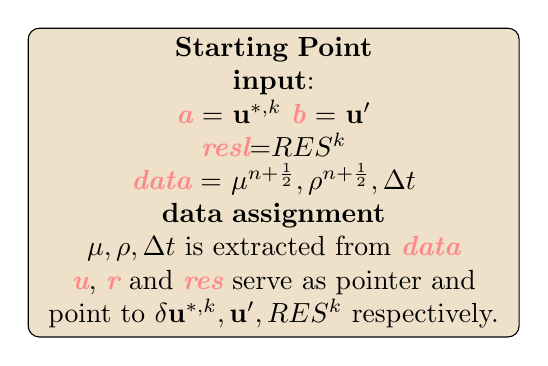
\begin{tikzpicture}
    \node [block](init){
        \textbf{Starting Point}\\
        \textbf{input}: \\
        \para{a} = $\mathbf{u}^{*,k}$ \para{b} = $ \mathbf{u}'$\\ \para{resl}=$RES^k$\\ \para{data} = $\mu^ {n+\frac{1}{2}}, \rho^{n+\frac{1}{2}}, \Delta t$\\
        \textbf{data assignment}\\
        $\mu,\rho,\Delta t$ is extracted from \para{data}\\
        \para{u}, \para{r} and \para{res} serve as pointer and point to $ \delta \mathbf{u}^{*,k}, \mathbf{u}', RES^k$ respectively.
      };
  \end{tikzpicture}
  \columnbreak
  \begin{minted}[obeytabs=false,mathescape=true,breaklines]{cpp}
static double residual_viscosity (scalar * a, scalar * b, scalar * resl, 
          void * data)
{
  struct Viscosity * p = (struct Viscosity *) data;
  (const) face vector mu = p->mu;
  (const) scalar rho = p->rho;
  double dt = p->dt;
  vector u = vector(a[0]), r = vector(b[0]), res = vector(resl[0]);
  double maxres = 0.;
  \end{minted}
\end{multicols}

\begin{center}
  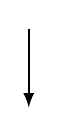
\begin{tikzpicture}
    \draw[-latex,thick](0,0) -- (0,-1); 
  \end{tikzpicture}
\end{center}

\begin{multicols}{2}
  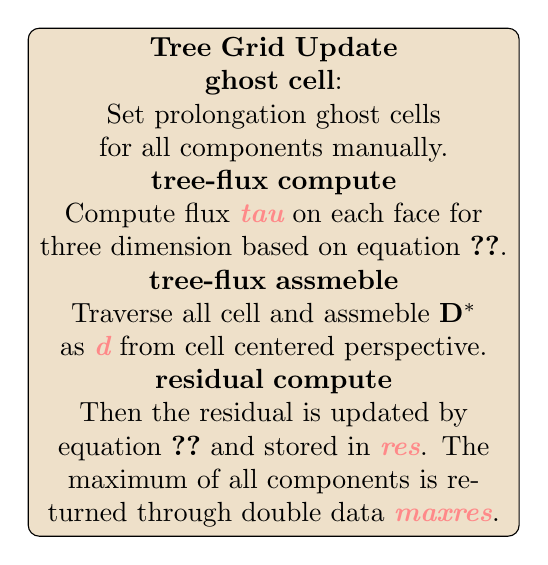
\begin{tikzpicture}
    \node [block](init){
        \textbf{Tree Grid Update}\\
        \textbf{ghost cell}: \\
        Set prolongation ghost cells for all components manually.\\
        \textbf{tree-flux compute}\\
        Compute flux \para{tau} on each face for three dimension based on equation \ref{equ:2dunfold}.\\
        \textbf{tree-flux assmeble}\\
        Traverse all cell and assmeble $ \mathbf{D}^*$ as \para{d} from cell centered perspective.\\
        \textbf{residual compute}\\
        Then the residual is updated by equation \ref{equ:resi} and stored in \para{res}. The maximum of all components is returned through double data \para{maxres}.
      };
  \end{tikzpicture}
  \columnbreak
  \begin{minted}[obeytabs=false,mathescape=true,breaklines]{cpp}
#if TREE
  boundary ({u});
  
  foreach_dimension() {
    face vector taux[];
    foreach_face(x)
      taux.x[] = 2.*mu.x[]*(u.x[] - u.x[-1])/Delta;
    #if dimension > 1
      foreach_face(y)
        taux.y[] = mu.y[]*(u.x[] - u.x[0,-1] + 
        (u.y[1,-1] + u.y[1,0])/4. -
        (u.y[-1,-1] + u.y[-1,0])/4.)/Delta;
    #endif
    #if dimension > 2
      foreach_face(z)
        taux.z[] = mu.z[]*(u.x[] - u.x[0,0,-1] + 
        (u.z[1,0,-1] + u.z[1,0,0])/4. -
        (u.z[-1,0,-1] + u.z[-1,0,0])/4.)/Delta;
    #endif
    foreach (reduction(max:maxres)) {
      double d = 0.;
      foreach_dimension()
        d += taux.x[1] - taux.x[];
        res.x[] = r.x[] - lambda.x*u.x[] + dt/rho[]*d/Delta;
      if (fabs (res.x[]) > maxres)
        maxres = fabs (res.x[]);
    }
  }
  \end{minted}
\end{multicols}

\begin{center}
  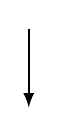
\begin{tikzpicture}
    \draw[-latex,thick](0,0) -- (0,-1); 
  \end{tikzpicture}
\end{center}

\begin{multicols}{2}
  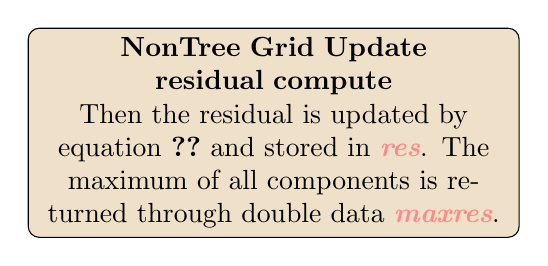
\begin{tikzpicture}
    \node [block](init){
        \textbf{NonTree Grid Update}\\
        \textbf{residual compute}\\
        Then the residual is updated by equation \ref{equ:resi} and stored in \para{res}. The maximum of all components is returned through double data \para{maxres}.
      };
  \end{tikzpicture}
  \columnbreak
  \begin{minted}[obeytabs=false,mathescape=true,breaklines]{cpp}
#else
  foreach (reduction(max:maxres))
    foreach_dimension() {
      res.x[] = r.x[] - lambda.x*u.x[] +
        dt/rho[]*(2.*mu.x[1,0]*(u.x[1] - u.x[])
        - 2.*mu.x[]*(u.x[] - u.x[-1])
  #if dimension > 1
        + mu.y[0,1]*(u.x[0,1] - u.x[] +
             (u.y[1,0] + u.y[1,1])/4. -
             (u.y[-1,0] + u.y[-1,1])/4.)
        - mu.y[]*(u.x[] - u.x[0,-1] +
            (u.y[1,-1] + u.y[1,0])/4. -
            (u.y[-1,-1] + u.y[-1,0])/4.)
	#endif
  #if dimension > 2
        + mu.z[0,0,1]*(u.x[0,0,1] - u.x[] +
           (u.z[1,0,0] + u.z[1,0,1])/4. -
           (u.z[-1,0,0] + u.z[-1,0,1])/4.)
        - mu.z[]*(u.x[] - u.x[0,0,-1] +
            (u.z[1,0,-1] + u.z[1,0,0])/4. -
            (u.z[-1,0,-1] + u.z[-1,0,0])/4.)
	#endif
		  )/sq(Delta);
      if (fabs (res.x[]) > maxres)
	maxres = fabs (res.x[]);
    }
#endif
  return maxres;
}

#undef lambda
  \end{minted}
\end{multicols}

\subsection{\func{viscosity}}
\subsubsection{Parameters}
\begin{center}
  \begin{tabular}{|c|c|c|c|c|}
    \hline
    Name & Data type & Status & Option/Default & Representation (before/after)\\[0.5ex]
    \hline\hline
    \rowcolor{output}\para{u} & vector & update & compulsory & $ \mathbf{u}'/ \mathbf{u}^*$\\
    \hline
    \para{mu} & face vector & unchanged & compulsory & $ \mu^{n+ \frac{1}{2}}$\\
    \hline
    \para{rho} & scalar & unchanged & compulsory & $\rho^{n+ \frac{1}{2}}$\\
    \hline
    \para{dt} & double & unchanged & compulsory & $\Delta t$ \\
    \hline
    \para{nrelax} & int & unchanged & optional/4 & $ max\, of \, iteration$ \\
    \hline
    \rowcolor{output}\para{res} & scalar* & \textbf{output} & optional/NULL & $RES$ \\
    \hline
  \end{tabular}
\end{center}

\subsubsection{Worth Mentioning Details}
The function to assemble all the tools built in this headfile or in 'poisson.h' and solve the governing equation equation \ref{equ:desired}. Details about implicit iteration solver construction used here are explored in 'poisson.h Documentation' which shall not be repeated again.

\subsubsection{Program Workflow}
\begin{multicols}{2}
  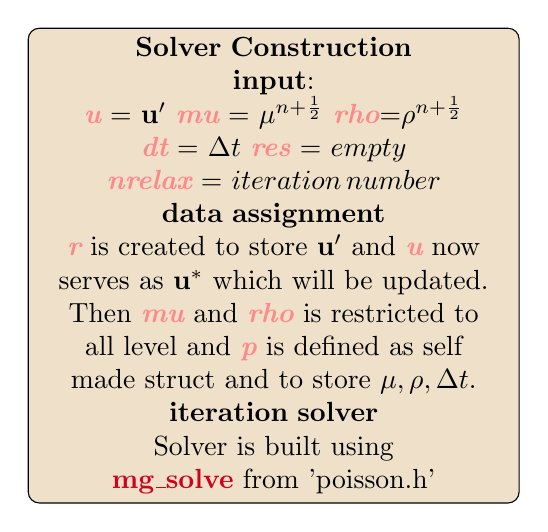
\begin{tikzpicture}
    \node [block](init){
        \textbf{Solver Construction}\\
        \textbf{input}: \\
        \para{u} = $\mathbf{u}'$ \para{mu} = $ \mu^{n+ \frac{1}{2}}$ \para{rho}=$\rho^{n+ \frac{1}{2}}$\\ \para{dt} = $ \Delta t$ \para{res} = $empty$\\ \para{nrelax} = $iteration\, number$\\
        \textbf{data assignment}\\
        \para{r} is created to store $ \mathbf{u}'$ and \para{u} now serves as $ \mathbf{u}^*$ which will be updated.\\ Then \para{mu} and \para{rho} is restricted to all level and \para{p} is defined as self made struct and to store $\mu,\rho,\Delta t$.\\
        \textbf{iteration solver}\\
        Solver is built using \func{mg\_solve} from 'poisson.h'
      };
  \end{tikzpicture}
  \columnbreak
  \begin{minted}[obeytabs=false,mathescape=true,breaklines]{cpp}
trace
mgstats viscosity (vector u, face vector mu, scalar rho, double dt, int nrelax = 4, scalar * res = NULL)
{
  vector r[];
  foreach()
    foreach_dimension()
      r.x[] = u.x[];

  restriction ({mu,rho});
  struct Viscosity p = { mu, rho, dt };
  return mg_solve ((scalar *){u}, (scalar *){r}, residual_viscosity, relax_viscosity, &p, nrelax, res);
}
  \end{minted}
\end{multicols}


\subsection{\func{viscosity\_explicit}}
\subsubsection{Parameters}
\begin{center}
  \begin{tabular}{|c|c|c|c|c|}
    \hline
    Name & Data type & Status & Option/Default & Representation (before/after)\\[0.5ex]
    \hline\hline
    \rowcolor{output}\para{u} & vector & update & compulsory & $ \mathbf{u}'/ \mathbf{u}^*$\\
    \hline
    \para{mu} & face vector & unchanged & compulsory & $ \mu^{n+ \frac{1}{2}}$\\
    \hline
    \para{rho} & scalar & unchanged & compulsory & $\rho^{n+ \frac{1}{2}}$\\
    \hline
    \para{dt} & double & unchanged & compulsory & $\Delta t$ \\
    \hline
  \end{tabular}
\end{center}

\subsubsection{Worth Mentioning Details}
Different from implicit form shown in equation \ref{equ:desired}, the governing equation of this function is explicit
\begin{equation}
  \rho_{n+ \frac{1}{2}}[ \frac{ \mathbf{u}^*- \mathbf{u}'}{\Delta t}] = \nabla\cdot [2\mu_{n+ \frac{1}{2}} \mathbf{D}']
\end{equation}
Then
\begin{equation}
  \mathbf{u}^* = \mathbf{u}' + \frac{\Delta t\nabla\cdot[2 \mu_{n+ \frac{1}{2}} \mathbf{D}']}{\rho_{n + \frac{1}{2}}} 
\end{equation}
According to Sec.\ref{sec:resi}, 
if \para{a}, \para{b} of \func{viscosity\_residual} are set to be the same and equal to $ \mathbf{u}'$ then the output yields
\begin{equation}
  RES = \frac{\Delta t\nabla\cdot[2 \mu_{n+ \frac{1}{2}} \mathbf{D}']}{\rho_{n + \frac{1}{2}}}
\end{equation}
Hence
\begin{equation}
  \mathbf{u}^* = \mathbf{u}' + \frac{\Delta t\nabla\cdot[2 \mu_{n+ \frac{1}{2}} \mathbf{D}']}{\rho_{n + \frac{1}{2}}}= \mathbf{u}'+ RES 
\end{equation}
\subsubsection{Program Workflow}
\begin{multicols}{2}
  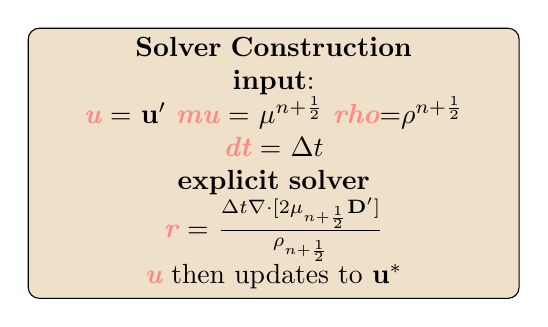
\begin{tikzpicture}
    \node [block](init){
        \textbf{Solver Construction}\\
        \textbf{input}: \\
        \para{u} = $\mathbf{u}'$ \para{mu} = $ \mu^{n+ \frac{1}{2}}$ \para{rho}=$\rho^{n+ \frac{1}{2}}$\\ \para{dt} = $ \Delta t$\\
        \textbf{explicit solver}\\
        \para{r} = $\frac{\Delta t\nabla\cdot[2 \mu_{n+ \frac{1}{2}} \mathbf{D}']}{\rho_{n + \frac{1}{2}}}$\\
        \para{u} then updates to $ \mathbf{u}^*$
      };
  \end{tikzpicture}
  \columnbreak
  \begin{minted}[obeytabs=false,mathescape=true,breaklines]{cpp}
trace
mgstats viscosity_explicit (vector u, face vector mu, scalar rho, double dt)
{
  vector r[];
  mgstats mg = {0};
  struct Viscosity p = { mu, rho, dt };
  mg.resb = residual_viscosity ((scalar *){u}, (scalar *){u}, (scalar *){r}, &p);
  foreach()
    foreach_dimension()
      u.x[] += r.x[];
  return mg;
}
  \end{minted}
\end{multicols}
\printbibliography
\end{document}
